\documentclass[a4paper]{book}
\usepackage{xeCJK}
\usepackage{verbatim}
\usepackage{graphicx}
\usepackage{hyperref}
\hypersetup{colorlinks}
%\setCJKmainfont{Noto Sans CJK SC}
\setCJKmainfont{宋体}
\setCJKmonofont{微软雅黑}
\pagestyle{plain}
\title{个人简历}
\author{周明东}
\begin{document}
	\frontmatter
	\maketitle
	%\include{preface}
	\tableofcontents

	\mainmatter
	\section{简单信息}
		\chapter{姓名与通信}
\begin{tabular}{ll}
\hline
  Name : & 周明东 \\
  Tel : & 13922835173 \\
  E-mail : & 505732590@qq.com \\
  GitHub : & \url{https://github.com/catRat} \\
  QQ : & 505732590 \\
  \hline
\end{tabular}

	\section{基本信息}
		\section{基本信息}
周明东, 男, 壮族, 于 1992 年农历七月, 全国贫困县之一的广西那坡县, 一个农场员工家庭中生, 小学时代当升旗手, 初中时代当领操, 学习委员, 班长, 经过付出努力, 获得了 09 年中考中 A+ 的总成绩, 并于当年被广西百色市百色民族高中录取, 成为了班里上市重点高中的 4 名同学之一; 高中时代当过物理科代表, 参加过班级乒乓球比赛, 13 年被广西河池学院录取; 大学时代在一次主题为"创业"的就业指导课中,在本小组中完成课堂作业任务中的 logo 设计(手绘); 17 年 11 月于深圳罗湖区参加工作, 就职于深圳市鸿安货运代理有限公司, 任北美航线价格部文员, 负责各船东在华中地区往北美航线的运输价格的更新以及鸿安集团各 Office 预定货量报表和一个合约年中从开始至今已完成货量报表的制作. 

	\section{技能}
		\begin{itemize}
\item 熟练使用 Window 操作系统, 了解 Linux 操作系统. 两年 Ubuntu 操作系统使用经验.
\item 熟练使用 Excel, 包括 Excel 的常用函数, Excel 的数据透视表.
\item 熟练使用 Word.
\item 熟练使用 PowerPoint.
\item 熟练使用 R, SPSS, Python.
\item 熟练使用 R 进行数据的清理, 包括
\begin{itemize}
\item 长格式与宽格式的转化,
\item 日期值处理,
\item 字符数据处理,
\end{itemize}
\item 熟练使用 R 的 ggplot2 完成数据可视化工作.
\item 熟练使用 SQL 语言.
\item 熟练使用 R 完成假设检验, 差异分析, 回归分析, 时间序列分析.
\item 了解 Shiny Server, 能够搭建 Shiny Server.
\end{itemize}

	\section{教育经历}
		\chapter{教育经历}
\begin{tabular}{ll}
  2013-2017 & 河池学院, 应用统计学, 专业课程是概率论和数理统计 \\
  2012-2013 & 广西百色市祈福高级中学 \\
  2009-2012 & 广西百色市百色民族高级中学  \\
  2007-2009 & 广西那坡县那坡民族初级中学  \\
  2005-2007 & 广西那坡县百合乡百合中学  \\
  1999-2005 & 广西那坡县百合乡那乐村那乐小学 \\
\end{tabular}

	%\section{Code Show}
		%利用 R 的数据结构和工具, 我能够高效地完成往往需要 VBA 才能完成的工作. 以下为为了完成某一数据处理工作而写的 R 脚本, 欢迎阅读. 我也可以写 Pyhont 脚本, 之所以不写, 是因为如果一个工具能够很好地完成某种任务, 为什么还要考虑其他工具? 

		%\verbatiminput{GetCode.R}	
		%\verbatiminput{GetId.R}	
		%\verbatiminput{Select.R}
		%\verbatiminput{blackcat.R}	
	\section{数据图作品展示}
		\begin{figure}
		\begin{center}
		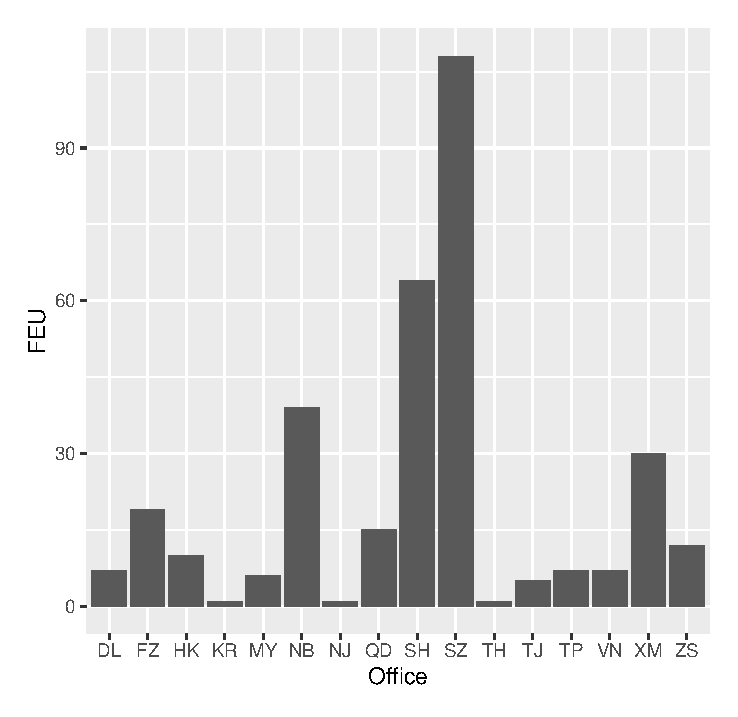
\includegraphics{Rplot01}
		\caption{带数据标签的着色的条形图}
		\end{center}
		\end{figure}
		\begin{figure}
		\begin{center}
		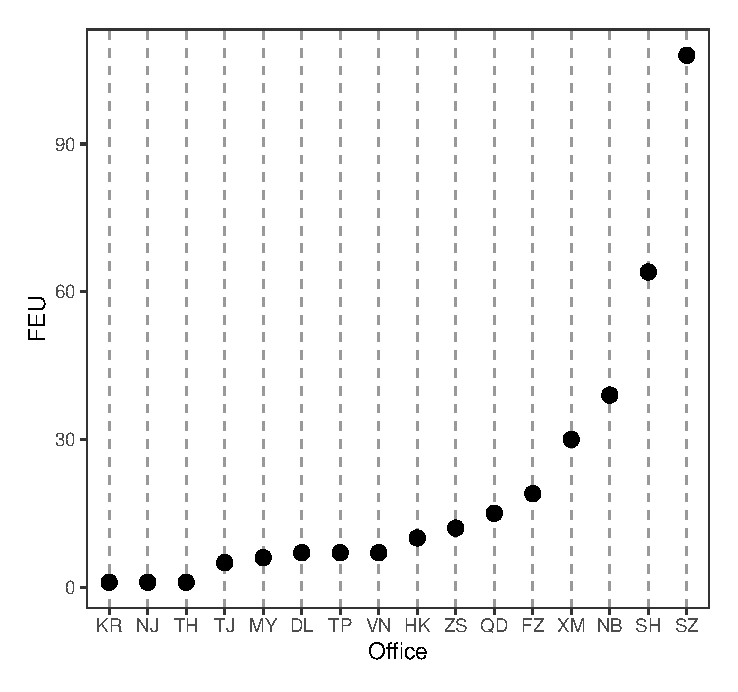
\includegraphics{Rplot13}
		\caption{用点的高度来替代条的高度}
		\end{center}
		\end{figure}
\end{document}
